   \begin{tikzpicture}
 \node at (0,0) {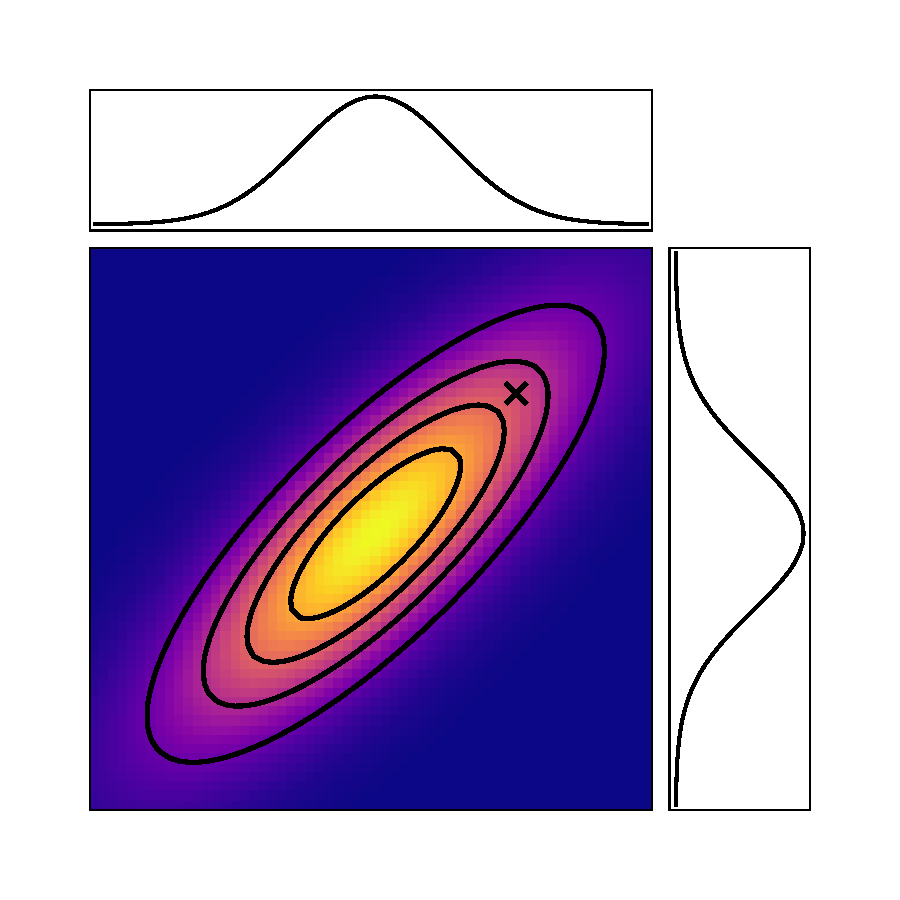
\includegraphics[scale=0.25]{test.pdf}};
    \def\xoffset{3.7}
    \def\yoffset{-1.2}
    \def\yoffsettwo{-0.75}
    \draw[line width = 0.25pt] (-1.53 + \xoffset,0.93 + \yoffset) rectangle (0.85 + \xoffset,1.52 + \yoffset) ;
    \draw[line width = 0.25pt] (-1.53 + \xoffset,0.93 + \yoffset + \yoffsettwo) rectangle (0.85 + \xoffset,1.52 + \yoffset + \yoffsettwo);

    \def\unifoffset{0.2}
    \def\unifoffsety{0.03}
    
    \draw[line width=0.5pt] (-1.53 + \xoffset, 0.96 + \yoffset + \unifoffsety) -- (-1.53 + \xoffset + \unifoffset, 0.96 + \yoffset+ \unifoffsety) --(-1.53 + \xoffset + \unifoffset, 1.4 + \yoffset+ \unifoffsety) -- (0.85 + \xoffset - \unifoffset , 1.4 + \yoffset+ \unifoffsety) -- (0.85 + \xoffset - \unifoffset , 0.96 + \yoffset+ \unifoffsety) -- (0.85 + \xoffset  , 0.96 + \yoffset+ \unifoffsety) ; 

    \draw[line width=0.5pt]  (-1.53 + \xoffset, 0.96 + \yoffset + \unifoffsety + \yoffsettwo) -- (-1.53 + \xoffset + \unifoffset, 0.96 + \yoffset+ \unifoffsety+ \yoffsettwo) --(-1.53 + \xoffset + \unifoffset, 1.4 + \yoffset+ \unifoffsety+ \yoffsettwo) -- (0.85 + \xoffset - \unifoffset , 1.4 + \yoffset+ \unifoffsety+ \yoffsettwo) -- (0.85 + \xoffset - \unifoffset , 0.96 + \yoffset+ \unifoffsety+ \yoffsettwo) -- (0.85 + \xoffset  , 0.96 + \yoffset+ \unifoffsety+ \yoffsettwo) ; 


    
    
    
    \node[draw, circle, scale = 1.4, fill=orange!15](1) at (1.85,-0.35){};
    \node[scale=0.65] at (1.85,-0.35) {$F_\mathcal{N}$};

    %\node[draw, scale=0.01](2) at (0.86,1.23) {};
    %\node[draw, scale=0.01](3) at (1.53,-0.35) {};
    %\draw[bend left =20, blue!30, line width = 0.3pt, scale = 0.1] (2) to (1);
    %\draw[bend left =20, blue!30, line width = 0.3pt, scale = 0.1] (3) to (1.180);
    
    \draw[thick, fill=OliveGreen, color=OliveGreen] (0.28,1.05) circle (0.022);
    \draw[thick, fill=black, color = NavyBlue] (1.06,0.24) circle (0.022);

    \draw[line width = 0.25, dashed] (0.28,0.24) -- (0.28,1.05);
    \draw[line width = 0.25, dashed] (0.28,0.24) -- (1.06,0.24);

    \draw[thick, fill=black, color = NavyBlue] (-1.4 + \xoffset + \unifoffset, 1.4 + \yoffset+ \unifoffsety+ \yoffsettwo) circle (0.022);
    \draw[thick, fill=black, color = OliveGreen] (0.3 + \xoffset + \unifoffset, 1.4 + \yoffset+ \unifoffsety) circle (0.022);

    \def\chixoffset{3.1}

     \node[draw, circle, scale = 1.4, fill=orange!15] at (1.85 + \chixoffset,-0.35){};
    \node[scale=0.65] at (1.85+ \chixoffset,-0.35) {$F_{\chi_d}^{-1}$};

    \draw[line width = 0.25pt] (-1.53 + \xoffset + \chixoffset,0.93 + \yoffset) rectangle (0.85 + \xoffset+ \chixoffset,1.52 + \yoffset) ;
    \draw[line width = 0.25pt] (-1.53 + \xoffset+ \chixoffset,0.93 + \yoffset + \yoffsettwo) rectangle (0.85 + \xoffset+ \chixoffset,1.52 + \yoffset + \yoffsettwo);

   

   % \node at (7,-2) {\includegraphics[scale=0.25]{chi2_test.pdf}};
    

    \def\arboffset{(5.5,-1.05)}

    \def \arboffsetx{5.29}
    \def\arboffsety{-0.25}
    
        
    \draw[line width = 0.5pt] [black] plot [smooth, tension=0.6] coordinates { (\arboffsetx,\arboffsety)(0.05+\arboffsetx,0.28+\arboffsety) (0.1+\arboffsetx,0.41+\arboffsety) (0.16+\arboffsetx,0.49+\arboffsety) (0.26+\arboffsetx,0.54+\arboffsety) (0.47+\arboffsetx,0.485+\arboffsety)(0.85+\arboffsetx,0.3+\arboffsety)(1.1+\arboffsetx,0.2+\arboffsety) (1.45+\arboffsetx,0.1+\arboffsety)(1.83+\arboffsetx,0.05+\arboffsety)(2.35+\arboffsetx,0.025+\arboffsety)} ;

    \draw[line width = 0.5pt] [black] plot [smooth, tension=0.6] coordinates { (\arboffsetx,\arboffsety + \yoffsettwo)(0.05+\arboffsetx,0.28+\arboffsety+ \yoffsettwo) (0.1+\arboffsetx,0.41+\arboffsety+ \yoffsettwo) (0.16+\arboffsetx,0.49+\arboffsety+ \yoffsettwo) (0.26+\arboffsetx,0.54+\arboffsety+ \yoffsettwo) (0.47+\arboffsetx,0.485+\arboffsety+ \yoffsettwo)(0.85+\arboffsetx,0.3+\arboffsety+ \yoffsettwo)(1.1+\arboffsetx,0.2+\arboffsety+ \yoffsettwo) (1.45+\arboffsetx,0.1+\arboffsety+ \yoffsettwo)(1.83+\arboffsetx,0.05+\arboffsety+ \yoffsettwo)(2.35+\arboffsetx,0.025+\arboffsety+ \yoffsettwo)} ;

    \draw[thick, fill=black, color = OliveGreen] (-0.14 + \xoffset + \unifoffset + \chixoffset, 1.0 + \yoffset+ \unifoffsety) circle (0.022);
     \draw[thick, fill=black, color = NavyBlue] (-1.65 + \xoffset + \unifoffset + \chixoffset, 1.25 + \yoffset+ \unifoffsety+ \yoffsettwo) circle (0.022);
    
    
    \end{tikzpicture}